% ============================================================================
% Lecture 02 (B01): Why Deep Learning for Economics and Finance?
% Deep Learning for Solving and Estimating Dynamic Models in Economics and Finance
% Course author: Simon Scheidegger
% ============================================================================

\documentclass[aspectratio=169,11pt]{beamer}

% ---------- Theme and colors ----------
\usecolortheme{dove}
\setbeamertemplate{navigation symbols}{}
\setbeamertemplate{footline}{%
  \hfill\usebeamerfont{page number in head/foot}%
  \usebeamercolor[fg]{normal text}%
  \insertframenumber\,/\,\inserttotalframenumber\kern1em\vskip4pt}
\setbeamerfont{frametitle}{size=\huge}

% ---------- Packages ----------
\usepackage[utf8]{inputenc}
\usepackage[T1]{fontenc}
\usepackage{amsmath,amssymb,amsfonts}
\usepackage{bm}
\usepackage{graphicx}
\usepackage{tikz}
\usetikzlibrary{shapes,arrows.meta,positioning,calc,fit,backgrounds,patterns,decorations.pathreplacing}
\usepackage{pgfplots}
\pgfplotsset{compat=1.18}
\usepackage{booktabs}
\usepackage{hyperref}
\usepackage{multicol}
\usepackage{xcolor}
\usepackage{algorithm}
\usepackage{algorithmic}

% ---------- Custom colors ----------
\definecolor{uzhblue}{rgb}{0,0,0.5}
\definecolor{uzhgreylight}{RGB}{236,238,241}
\definecolor{uzhgreydark}{RGB}{81,86,94}
\definecolor{harvardcrimson}{RGB}{153,0,0}
\definecolor{unil@blue}{RGB}{0,140,204}
\definecolor{unil@black}{RGB}{35,31,32}
\definecolor{darkgreen}{RGB}{0,100,0}
\definecolor{darkred}{RGB}{139,0,0}
\definecolor{softblue}{RGB}{70,130,180}
\definecolor{softorange}{RGB}{230,159,0}
\definecolor{softgreen}{RGB}{0,158,115}

% ---------- Set beamer colors ----------
\setbeamercolor{frametitle}{bg=uzhgreylight, fg=uzhblue}
\setbeamercolor{title}{fg=uzhblue}
\setbeamercolor{structure}{fg=uzhblue}
\setbeamercolor{block title}{bg=unil@blue, fg=white}
\setbeamercolor{block body}{bg=uzhgreylight}
\setbeamercolor{block title alerted}{bg=darkred,fg=white}
\setbeamercolor{block body alerted}{bg=red!5}
\setbeamercolor{block title example}{bg=darkgreen,fg=white}
\setbeamercolor{block body example}{bg=green!5}
\setbeamercolor{item}{fg=unil@black}
\setbeamercolor{normal text}{fg=unil@black}

% ---------- Emphasis and hyperlinks ----------
\newcommand{\emphc}[1]{\textcolor{harvardcrimson}{#1}}
\hypersetup{colorlinks,linkcolor=harvardcrimson,urlcolor=harvardcrimson}

% ---------- Math commands ----------
\newcommand{\x}{\bm{x}}
\newcommand{\w}{\bm{w}}
\newcommand{\bb}{\bm{b}}
\newcommand{\z}{\bm{z}}
\newcommand{\W}{\bm{W}}
\newcommand{\X}{\bm{X}}
\renewcommand{\a}{\bm{a}}
\newcommand{\R}{\mathbb{R}}
\newcommand{\E}[1]{\mathbb{E}\!\left[#1\right]}
\DeclareMathOperator*{\argmin}{arg\,min}
\DeclareMathOperator*{\argmax}{arg\,max}

\title[Lecture 03 (B02)]{Lecture 03 (B02): Training Neural Networks}
\subtitle{Architecture, gradients, optimization, regularization-adjacent mechanics}
\author{Simon Scheidegger}
\institute{HEC, University of Lausanne}
\date{}
\begin{document}

{\setbeamercolor{background canvas}{bg=uzhgreylight}
\begin{frame}
\titlepage
\end{frame}
}

\begin{frame}{}
\begin{columns}[c]
\column{0.65\textwidth}
\begin{center}
{\Huge \textcolor{uzhblue}{Part II}}\\[0.8em]
{\LARGE From Perceptrons to Deep Networks}
\end{center}
\column{0.30\textwidth}
\begin{center}

\includegraphics[width=0.7\textwidth]{figures/r2d2.png}
\end{center}
\end{columns}
\end{frame}

% --- Biological Neurons ---
\begin{frame}{Biological Neurons}
\begin{columns}[T]
\column{0.55\textwidth}
\begin{center}

\includegraphics[width=\textwidth]{figures/neurons.png}
\end{center}

\column{0.42\textwidth}
\textbf{The brain} is a massively parallel computer made of $\sim$86 billion neurons.

\vspace{0.3cm}
Each neuron:
\begin{itemize}
    \item Receives signals via \textbf{dendrites}
    \item Integrates signals in the \textbf{cell body}
    \item Transmits output along the \textbf{axon}
    \item Communicates at \textbf{synapses}
\end{itemize}

\vspace{0.3cm}
{\small Artificial neural networks are a \textit{very loose} abstraction of this biological architecture.}
\end{columns}
\end{frame}

% --- Slide 16: McCulloch-Pitts Neuron ---
\begin{frame}{The Artificial Neuron (McCulloch \& Pitts, 1943)}
{\small\emphc{From biology to math:} turn the neuron on the previous slide into an equation, synapses become weights $w_i$, dendritic inputs become $x_i$, the soma's integration becomes a sum, and firing becomes a nonlinear activation.}
\vspace{0.2cm}
\begin{columns}[T]
\column{0.55\textwidth}
\begin{center}
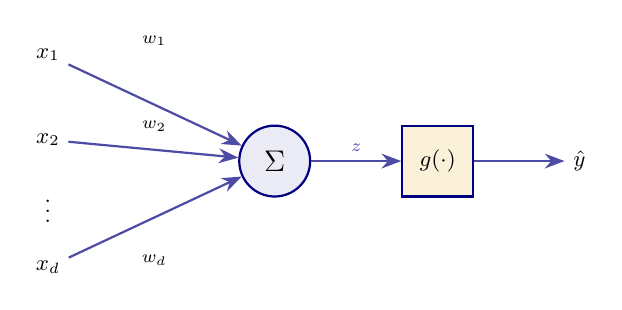
\begin{tikzpicture}[scale=0.9, transform shape,
    neuron/.style={circle, draw=uzhblue, thick, minimum size=10mm, fill=uzhblue!8},
    arr/.style={-{Stealth[length=2.5mm]}, thick, uzhblue!70}]

    % Inputs
    \node[font=\small] (x1) at (0,2) {$x_1$};
    \node[font=\small] (x2) at (0,0.8) {$x_2$};
    \node[font=\small] at (0,-0.1) {$\vdots$};
    \node[font=\small] (xm) at (0,-1) {$x_d$};

    % Weights
    \node[font=\scriptsize, above] at (1.5,2) {$w_1$};
    \node[font=\scriptsize, above] at (1.5,0.8) {$w_2$};
    \node[font=\scriptsize, below] at (1.5,-0.7) {$w_d$};

    % Sum node
    \node[neuron, font=\large] (sum) at (3.2,0.5) {$\Sigma$};

    % Activation
    \node[rectangle, draw=uzhblue, thick, fill=softorange!15,
          minimum width=10mm, minimum height=10mm, font=\small] (act) at (5.5,0.5) {$g(\cdot)$};

    % Output
    \node[font=\small] (out) at (7.5,0.5) {$\hat{y}$};

    % Arrows
    \draw[arr] (x1) -- (sum);
    \draw[arr] (x2) -- (sum);
    \draw[arr] (xm) -- (sum);
    \draw[arr] (sum) -- node[above, font=\scriptsize]{$z$} (act);
    \draw[arr] (act) -- (out);
\end{tikzpicture}
\end{center}

\column{0.42\textwidth}
Three components:
\begin{enumerate}
    \item \textbf{Weighted inputs} $w_i$ (synaptic weights)
    \item \textbf{Summation:} $z = \sum_{j=1}^{d} w_j x_j$
    \item \textbf{Activation} $g(z)$: nonlinear function determining whether the neuron ``fires''
\end{enumerate}

\vspace{0.3cm}
{\small Original model used a step function as activation. Modern networks use smooth alternatives.}
\end{columns}
\end{frame}

% --- Hebb's Rule ---
\begin{frame}{Hebb's Rule (1949)}
{\small\emphc{The missing ingredient --- learning:} the McCulloch--Pitts neuron is static; its weights $w_i$ are fixed by hand. Hebb asks \textit{how should the weights change with experience?}}
\vspace{0.2cm}
\begin{columns}[T]
\column{0.55\textwidth}
\textbf{``Neurons that fire together, wire together.''}

\vspace{0.3cm}
Donald Hebb proposed that if neuron $A$ repeatedly causes neuron $B$ to fire, the synapse from $A$ to $B$ is strengthened:
\[
    \Delta w_{ij} = \eta\, x_i\, y_j
\]

\vspace{0.3cm}
This is the foundation of learning rules in artificial neural networks.

\vspace{0.3cm}
{\small Analogy: every time you eat chocolate and feel happy, the association between ``chocolate'' and ``happiness'' neurons strengthens!}

\column{0.40\textwidth}
\begin{center}

\includegraphics[width=\textwidth]{figures/chocolate.png}
\end{center}
\end{columns}
\end{frame}

% --- Slide 17: The Perceptron ---
\begin{frame}{The Perceptron}
\begin{columns}[T]
\column{0.48\textwidth}
\begin{center}
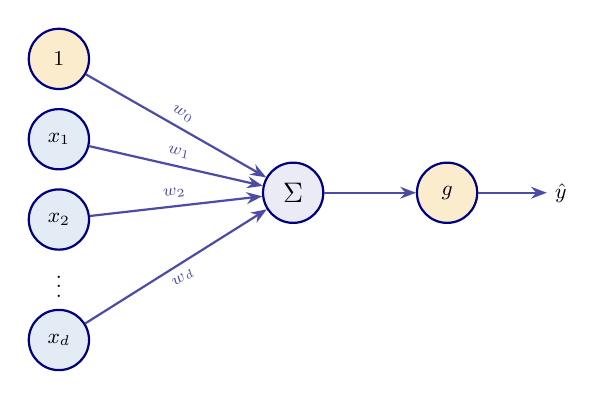
\begin{tikzpicture}[scale=0.85, transform shape,
    neuron/.style={circle, draw=uzhblue, thick, minimum size=9mm, fill=uzhblue!8},
    arr/.style={-{Stealth[length=2mm]}, thick, uzhblue!70}]

    % Bias
    \node[neuron, fill=softorange!20, font=\small] (b) at (0,3) {$1$};
    \node[neuron, fill=softblue!15, font=\small] (x1) at (0,1.8) {$x_1$};
    \node[neuron, fill=softblue!15, font=\small] (x2) at (0,0.6) {$x_2$};
    \node[font=\small] at (0,-0.3) {$\vdots$};
    \node[neuron, fill=softblue!15, font=\small] (xd) at (0,-1.2) {$x_d$};

    % Sum
    \node[neuron, font=\large] (sum) at (3.5,1) {$\Sigma$};

    % Activation
    \node[neuron, fill=softorange!20, font=\small] (act) at (5.8,1) {$g$};

    % Output
    \node[font=\small] (out) at (7.5,1) {$\hat{y}$};

    % Weight labels
    \draw[arr] (b) -- node[above, font=\scriptsize, sloped]{$w_0$} (sum);
    \draw[arr] (x1) -- node[above, font=\scriptsize, sloped]{$w_1$} (sum);
    \draw[arr] (x2) -- node[above, font=\scriptsize, sloped]{$w_2$} (sum);
    \draw[arr] (xd) -- node[below, font=\scriptsize, sloped]{$w_d$} (sum);
    \draw[arr] (sum) -- (act);
    \draw[arr] (act) -- (out);
\end{tikzpicture}
\end{center}

\column{0.48\textwidth}
\textbf{Forward pass:}
\[
    \hat{y} \;=\; g\!\left(w_0 + \sum_{j=1}^{d} x_j\, w_j\right)
\]

In vector notation, with $\w = (w_1,\dots,w_d)^\top$:
\[
    \hat{y} \;=\; g\!\big(w_0 + \x^\top \w\big)
\]

\vspace{0.2cm}
\begin{itemize}
    \item $w_0$ is the \textbf{bias} (shifts activation)
    \item $g(\cdot)$ is a nonlinear \textbf{activation function}
\end{itemize}
\end{columns}
\end{frame}

% --- Slide 18: Forward Propagation Vector Form ---
\begin{frame}{Forward Propagation -- Vector Form}
Absorbing the bias into the weight vector, define
$\tilde{\x} = (1, x_1, \dots, x_d)^\top \in \R^{d+1}$ and
$\tilde{\w} = (w_0, w_1, \dots, w_d)^\top \in \R^{d+1}$. Then:
\[
    \boxed{\hat{y} \;=\; g\!\big(\tilde{\x}^\top \tilde{\w}\big)}
\]

\vspace{0.5cm}
\begin{block}{Key insight}
The perceptron computes a \textbf{weighted linear combination} of its inputs, applies a \textbf{nonlinearity}, and produces a scalar output.  Without $g$, this is just linear regression.
\end{block}

\vspace{0.3cm}
{\small We will use the notation $z = \w^\top\x + b$ (separating bias $b$ from weights $\w$) for the remainder of this lecture.}
\end{frame}

% --- Slide 19: Activation Functions ---
\begin{frame}{Activation Functions}
\begin{center}
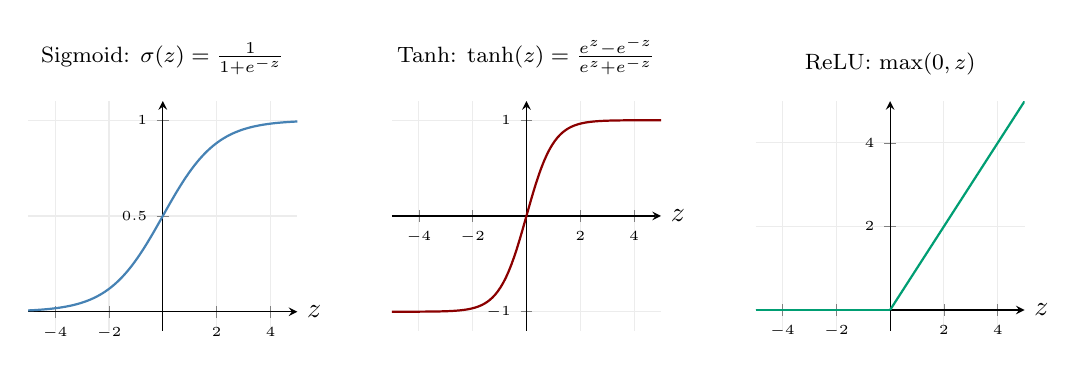
\begin{tikzpicture}
\begin{axis}[
    name=plot1,
    width=5cm, height=4.5cm,
    title={\footnotesize Sigmoid: $\sigma(z) = \frac{1}{1+e^{-z}}$},
    title style={font=\footnotesize},
    xlabel={$z$}, xlabel style={font=\tiny},
    tick label style={font=\tiny},
    xmin=-5, xmax=5, ymin=-0.1, ymax=1.1,
    grid=major, grid style={gray!15},
    axis lines=middle,
    every axis x label/.style={at={(current axis.right of origin)}, anchor=west},
    every axis y label/.style={at={(current axis.above origin)}, anchor=south},
]
    \addplot[thick, softblue, domain=-5:5, samples=100]{1/(1+exp(-x))};
\end{axis}

\begin{axis}[
    at={($(plot1.east)+(1.2cm,0)$)}, anchor=west,
    name=plot2,
    width=5cm, height=4.5cm,
    title={\footnotesize Tanh: $\tanh(z) = \frac{e^z - e^{-z}}{e^z + e^{-z}}$},
    title style={font=\footnotesize},
    xlabel={$z$}, xlabel style={font=\tiny},
    tick label style={font=\tiny},
    xmin=-5, xmax=5, ymin=-1.2, ymax=1.2,
    grid=major, grid style={gray!15},
    axis lines=middle,
    every axis x label/.style={at={(current axis.right of origin)}, anchor=west},
    every axis y label/.style={at={(current axis.above origin)}, anchor=south},
]
    \addplot[thick, darkred, domain=-5:5, samples=100]{tanh(x)};
\end{axis}

\begin{axis}[
    at={($(plot2.east)+(1.2cm,0)$)}, anchor=west,
    width=5cm, height=4.5cm,
    title={\footnotesize ReLU: $\max(0, z)$},
    title style={font=\footnotesize},
    xlabel={$z$}, xlabel style={font=\tiny},
    tick label style={font=\tiny},
    xmin=-5, xmax=5, ymin=-0.5, ymax=5,
    grid=major, grid style={gray!15},
    axis lines=middle,
    every axis x label/.style={at={(current axis.right of origin)}, anchor=west},
    every axis y label/.style={at={(current axis.above origin)}, anchor=south},
]
    \addplot[thick, softgreen, domain=-5:0, samples=2]{0};
    \addplot[thick, softgreen, domain=0:5, samples=2]{x};
\end{axis}
\end{tikzpicture}
\end{center}

\vspace{-0.1cm}
\begin{center}
\begin{small}
\begin{tabular}{lccc}
\toprule
& \textbf{Sigmoid} & \textbf{Tanh} & \textbf{ReLU} \\
\midrule
Range & $(0,1)$ & $(-1,1)$ & $[0,\infty)$ \\
$g'(z)$ & $\sigma(z)(1-\sigma(z))$ & $1 - \tanh^2(z)$ & $\begin{cases}1&z>0\\0&z<0\end{cases}$ \\
\bottomrule
\end{tabular}
\end{small}
\end{center}
\end{frame}

% --- Slide 20: Why Nonlinearity? ---
\begin{frame}{Why Nonlinearity Matters}
\begin{columns}[T]
\column{0.47\textwidth}
\begin{center}
{\small\textbf{Linear activation} $\Rightarrow$ linear boundary}
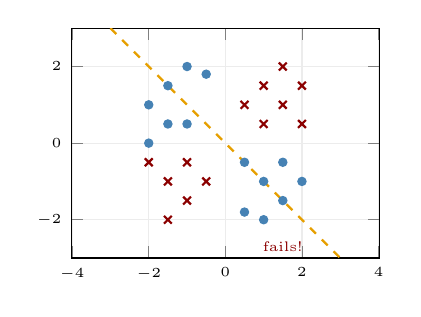
\begin{tikzpicture}
\begin{axis}[
    width=5.5cm, height=4.5cm,
    tick label style={font=\tiny},
    xmin=-3, xmax=3, ymin=-3, ymax=3,
    grid=major, grid style={gray!15},
    axis equal,
]
    % Two spirals (simplified as overlapping clusters)
    \addplot[only marks, mark=*, mark size=1.5pt, softblue] coordinates {
        (-2,1) (-1.5,1.5) (-1,2) (-0.5,1.8) (-1.5,0.5) (-2,0) (-1,0.5)
        (0.5,-1.8) (1,-2) (1.5,-1.5) (2,-1) (1.5,-0.5) (1,-1) (0.5,-0.5)
    };
    \addplot[only marks, mark=x, mark size=2pt, darkred, thick] coordinates {
        (1,1.5) (1.5,1) (2,0.5) (1.5,2) (0.5,1) (1,0.5) (2,1.5)
        (-1,-1.5) (-1.5,-1) (-2,-0.5) (-1.5,-2) (-0.5,-1) (-1,-0.5)
    };
    % Linear boundary (fails)
    \addplot[thick, softorange, dashed, domain=-3:3]{-x};
    \node[font=\tiny, darkred] at (axis cs:1.5,-2.7) {fails!};
\end{axis}
\end{tikzpicture}
\end{center}

\column{0.47\textwidth}
\begin{center}
{\small\textbf{Nonlinear activation} $\Rightarrow$ curved boundary}
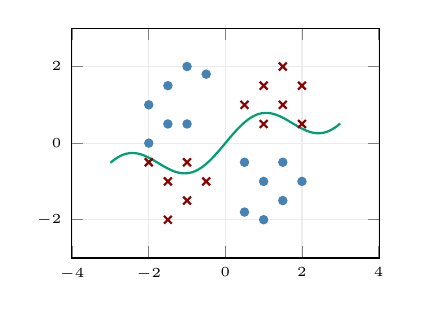
\begin{tikzpicture}
\begin{axis}[
    width=5.5cm, height=4.5cm,
    tick label style={font=\tiny},
    xmin=-3, xmax=3, ymin=-3, ymax=3,
    grid=major, grid style={gray!15},
    axis equal,
]
    \addplot[only marks, mark=*, mark size=1.5pt, softblue] coordinates {
        (-2,1) (-1.5,1.5) (-1,2) (-0.5,1.8) (-1.5,0.5) (-2,0) (-1,0.5)
        (0.5,-1.8) (1,-2) (1.5,-1.5) (2,-1) (1.5,-0.5) (1,-1) (0.5,-0.5)
    };
    \addplot[only marks, mark=x, mark size=2pt, darkred, thick] coordinates {
        (1,1.5) (1.5,1) (2,0.5) (1.5,2) (0.5,1) (1,0.5) (2,1.5)
        (-1,-1.5) (-1.5,-1) (-2,-0.5) (-1.5,-2) (-0.5,-1) (-1,-0.5)
    };
    % Nonlinear boundary
    \addplot[thick, softgreen, domain=-3:3, samples=100]{0.5*sin(deg(x*1.8))+0.3*x};
\end{axis}
\end{tikzpicture}
\end{center}
\end{columns}

\vspace{0.4cm}
\begin{alertblock}{Mathematical reason}
A composition of linear maps is still linear: $\W_2(\W_1\x+\bb_1)+\bb_2 = \W_2\W_1\x + (\W_2\bb_1+\bb_2)$.
Without nonlinearities, depth is useless.
\end{alertblock}
\end{frame}

% --- Slide 21: Perceptron Example ---
\begin{frame}{Perceptron -- A Worked Example}
\begin{columns}[T]
\column{0.50\textwidth}
Suppose we have trained weights $w_0=1$, $\w=(3, -2)^\top$, and sigmoid activation $\sigma$.

\vspace{0.3cm}
\textbf{Output:}
\[
    \hat{y} = \sigma(w_0 + \x^\top\w) = \sigma(1 + 3x_1 - 2x_2)
\]

For a new point $\x = (-1, 2)^\top$:
\begin{align*}
    z &= 1 + 3\cdot(-1) - 2\cdot 2 = -6 \\
    \hat{y} &= \sigma(-6) \approx 0.0025
\end{align*}

The discriminant line $1+3x_1-2x_2=0$ separates the two classes.

\column{0.47\textwidth}
\begin{center}
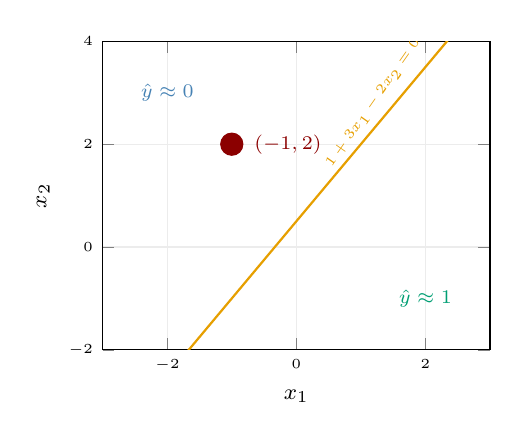
\begin{tikzpicture}
\begin{axis}[
    width=6.5cm, height=5.5cm,
    xlabel={$x_1$}, ylabel={$x_2$},
    xlabel style={font=\footnotesize},
    ylabel style={font=\footnotesize},
    tick label style={font=\tiny},
    xmin=-3, xmax=3, ymin=-2, ymax=4,
    grid=major, grid style={gray!15},
]
    % Decision boundary: 1 + 3x1 - 2x2 = 0 => x2 = 0.5 + 1.5*x1
    \addplot[thick, softorange, domain=-3:3, samples=2]{0.5 + 1.5*x};
    % New point
    \addplot[only marks, mark=*, mark size=4pt, darkred] coordinates {(-1,2)};
    \node[font=\scriptsize, darkred, right] at (axis cs:-0.8,2) {$(-1,2)$};
    % Region labels
    \node[font=\scriptsize, softblue] at (axis cs:-2,3) {$\hat{y} \approx 0$};
    \node[font=\scriptsize, softgreen] at (axis cs:2,-1) {$\hat{y} \approx 1$};
    % Boundary label
    \node[font=\tiny, softorange, rotate=55] at (axis cs:1.2,2.8) {$1+3x_1-2x_2=0$};
\end{axis}
\end{tikzpicture}
\end{center}
\end{columns}
\end{frame}

% --- Slide 22: Multi-Output Perceptron ---
\begin{frame}{Multi-Output Perceptron}
\begin{columns}[T]
\column{0.50\textwidth}
\begin{center}
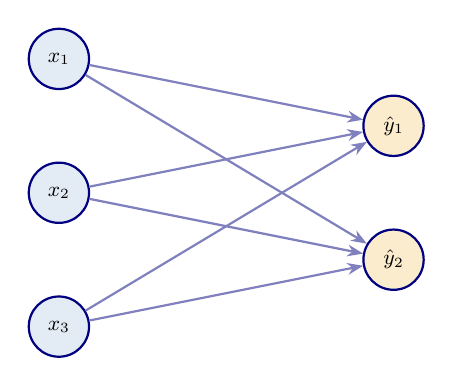
\begin{tikzpicture}[scale=0.85, transform shape,
    neuron/.style={circle, draw=uzhblue, thick, minimum size=9mm, fill=uzhblue!8},
    arr/.style={-{Stealth[length=2mm]}, thick, uzhblue!50}]

    % Inputs
    \node[neuron, fill=softblue!15, font=\small] (x1) at (0,2) {$x_1$};
    \node[neuron, fill=softblue!15, font=\small] (x2) at (0,0) {$x_2$};
    \node[neuron, fill=softblue!15, font=\small] (x3) at (0,-2) {$x_3$};

    % Outputs
    \node[neuron, fill=softorange!20, font=\small] (y1) at (5,1) {$\hat{y}_1$};
    \node[neuron, fill=softorange!20, font=\small] (y2) at (5,-1) {$\hat{y}_2$};

    % Connections
    \foreach \i in {x1,x2,x3} {
        \foreach \j in {y1,y2} {
            \draw[arr] (\i) -- (\j);
        }
    }
\end{tikzpicture}
\end{center}

\column{0.47\textwidth}
Each output unit computes its own weighted sum:
\[
    z_k = b_k + \sum_{j=1}^{d} w_{jk}\, x_j, \quad k=1,\dots,K
\]

In matrix form:
\[
    \z = \W\x + \bb, \qquad \hat{\bm{y}} = g(\z)
\]

where $\W\in\R^{K\times d}$ (one row per output unit) and $\bb\in\R^{K}$.  The same row-per-output convention is used in every later layer of this deck, so the formula extends directly to deep networks (slides 23--24).

\vspace{0.3cm}
{\small Each output has its own set of weights but shares the same inputs.}
\end{columns}
\end{frame}

% --- Slide 23: Single Hidden Layer ---
\begin{frame}{Single Hidden Layer Network}
\begin{columns}[T]
\column{0.48\textwidth}
\begin{center}
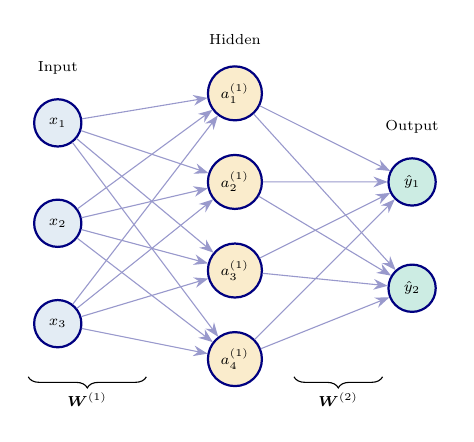
\begin{tikzpicture}[scale=0.75, transform shape,
    neuron/.style={circle, draw=uzhblue, thick, minimum size=8mm},
    arr/.style={-{Stealth[length=1.8mm]}, uzhblue!40}]

    % Input layer
    \node[neuron, fill=softblue!15, font=\scriptsize] (x1) at (0,2.5) {$x_1$};
    \node[neuron, fill=softblue!15, font=\scriptsize] (x2) at (0,0.8) {$x_2$};
    \node[neuron, fill=softblue!15, font=\scriptsize] (x3) at (0,-0.9) {$x_3$};

    % Hidden layer
    \node[neuron, fill=softorange!20, font=\scriptsize] (h1) at (3,3) {$a_1^{(1)}$};
    \node[neuron, fill=softorange!20, font=\scriptsize] (h2) at (3,1.5) {$a_2^{(1)}$};
    \node[neuron, fill=softorange!20, font=\scriptsize] (h3) at (3,0) {$a_3^{(1)}$};
    \node[neuron, fill=softorange!20, font=\scriptsize] (h4) at (3,-1.5) {$a_4^{(1)}$};

    % Output layer
    \node[neuron, fill=softgreen!20, font=\scriptsize] (y1) at (6,1.5) {$\hat{y}_1$};
    \node[neuron, fill=softgreen!20, font=\scriptsize] (y2) at (6,-0.3) {$\hat{y}_2$};

    % Connections
    \foreach \i in {x1,x2,x3} {
        \foreach \j in {h1,h2,h3,h4} { \draw[arr] (\i) -- (\j); }
    }
    \foreach \i in {h1,h2,h3,h4} {
        \foreach \j in {y1,y2} { \draw[arr] (\i) -- (\j); }
    }

    % Labels
    \node[font=\scriptsize, above] at (0,3.2) {Input};
    \node[font=\scriptsize, above] at (3,3.7) {Hidden};
    \node[font=\scriptsize, above] at (6,2.2) {Output};

    % Weight labels
    \draw[decorate, decoration={brace, amplitude=4pt, mirror}] (-0.5,-1.8) -- (1.5,-1.8)
        node[midway, below=4pt, font=\scriptsize]{$\W^{(1)}$};
    \draw[decorate, decoration={brace, amplitude=4pt, mirror}] (4,-1.8) -- (5.5,-1.8)
        node[midway, below=4pt, font=\scriptsize]{$\W^{(2)}$};
\end{tikzpicture}
\end{center}

\column{0.48\textwidth}
\textbf{Hidden layer:}
\begin{align*}
    \z^{(1)} &= \W^{(1)}\x + \bb^{(1)} \\
    \a^{(1)} &= g\!\big(\z^{(1)}\big)
\end{align*}

\textbf{Output layer:}
\begin{align*}
    \z^{(2)} &= \W^{(2)}\a^{(1)} + \bb^{(2)} \\
    \hat{\bm{y}} &= g_{\text{out}}\!\big(\z^{(2)}\big)
\end{align*}

where $\W^{(1)}\in\R^{n_1\times d}$, $\W^{(2)}\in\R^{K\times n_1}$.

\vspace{0.3cm}
{\small The hidden layer creates a \textbf{learned representation} of the input that the output layer then uses for prediction.}
\end{columns}
\end{frame}

% --- Slide 24: Deep Feedforward Network ---
\begin{frame}{Deep Feedforward Networks}
\begin{center}
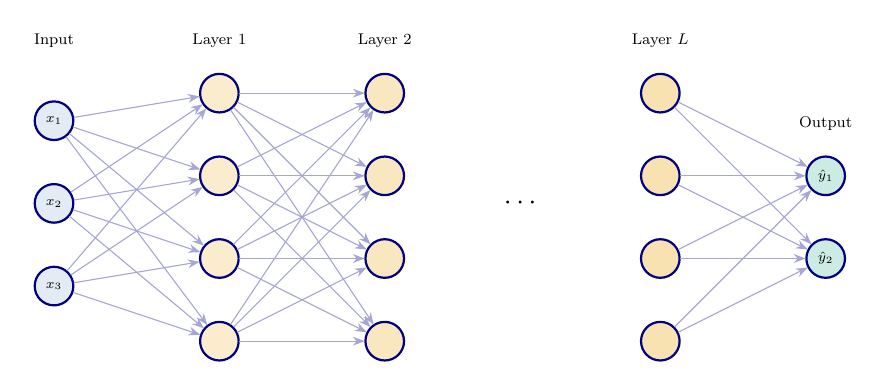
\begin{tikzpicture}[scale=0.7, transform shape,
    neuron/.style={circle, draw=uzhblue, thick, minimum size=7mm},
    arr/.style={-{Stealth[length=1.5mm]}, uzhblue!35}]

    % Input layer
    \foreach \i/\y in {1/2,2/0.5,3/-1} {
        \node[neuron, fill=softblue!15, font=\scriptsize] (x\i) at (0,\y) {$x_\i$};
    }
    % Hidden 1
    \foreach \i/\y in {1/2.5,2/1,3/-0.5,4/-2} {
        \node[neuron, fill=softorange!20, font=\tiny] (h1\i) at (3,\y) {};
    }
    % Hidden 2
    \foreach \i/\y in {1/2.5,2/1,3/-0.5,4/-2} {
        \node[neuron, fill=softorange!25, font=\tiny] (h2\i) at (6,\y) {};
    }
    % Hidden L
    \foreach \i/\y in {1/2.5,2/1,3/-0.5,4/-2} {
        \node[neuron, fill=softorange!30, font=\tiny] (hL\i) at (11,\y) {};
    }
    % Output
    \foreach \i/\y in {1/1,2/-0.5} {
        \node[neuron, fill=softgreen!20, font=\scriptsize] (y\i) at (14,\y) {$\hat{y}_\i$};
    }

    % Dots
    \node[font=\Large] at (8.5,0.5) {$\cdots$};

    % Connections
    \foreach \i in {1,2,3} { \foreach \j in {1,2,3,4} { \draw[arr] (x\i)--(h1\j); }}
    \foreach \i in {1,2,3,4} { \foreach \j in {1,2,3,4} { \draw[arr] (h1\i)--(h2\j); }}
    \foreach \i in {1,2,3,4} { \foreach \j in {1,2} { \draw[arr] (hL\i)--(y\j); }}

    % Layer labels
    \node[font=\footnotesize, above] at (0,3.2) {Input};
    \node[font=\footnotesize, above] at (3,3.2) {Layer 1};
    \node[font=\footnotesize, above] at (6,3.2) {Layer 2};
    \node[font=\footnotesize, above] at (11,3.2) {Layer $L$};
    \node[font=\footnotesize, above] at (14,1.7) {Output};
\end{tikzpicture}
\end{center}

\vspace{0.1cm}
An $L$-layer network computes a nested composition:
\[
    \boxed{f(\x;\bm{\theta}) = g_L\!\Big(\W^{(L)} g_{L-1}\!\big(\cdots g_1\!\big(\W^{(1)}\x + \bb^{(1)}\big)\cdots + \bb^{(L-1)}\big) + \bb^{(L)}\Big)}
\]

{\small Each layer transforms the representation.  \textbf{Depth} provides exponential gains in representational power over width alone.}
\end{frame}

% --- Slide 25: Universal Approximation ---
\begin{frame}{Universal Approximation Theorem}
\small
\begin{block}{Theorem (Cybenko 1989; Hornik, Stinchcombe \& White 1989)}
Let $g:\R\to\R$ be a bounded, non-constant, continuous activation function.  Then for any continuous function $f:\mathcal{K}\to\R$ on a compact set $\mathcal{K}\subset\R^d$ and any $\varepsilon>0$, there exists a single-hidden-layer network
\[
    F(\x) = \sum_{j=1}^{n_1} v_j\, g\!\big(\w_j^\top\x + b_j\big)
\]
such that $\sup_{\x\in\mathcal{K}} |F(\x) - f(\x)| < \varepsilon$.
\end{block}

\vspace{0.25cm}
\textbf{Caveats:}
\begin{itemize}\itemsep0pt
    \item The required width $n_1$ may be \textbf{exponentially large} in $d$.
    \item Existence $\neq$ efficient learnability.
    \item Practical success of deep learning suggests that \textbf{depth} provides a much more efficient parameterization than width alone.
\end{itemize}
\end{frame}

% --- Slide 26: Geometric View ---
\begin{frame}{A Geometric View: Learning to Untangle}
Neural networks learn \textbf{successive coordinate transformations} that make the data linearly separable.

\vspace{0.3cm}
\begin{center}
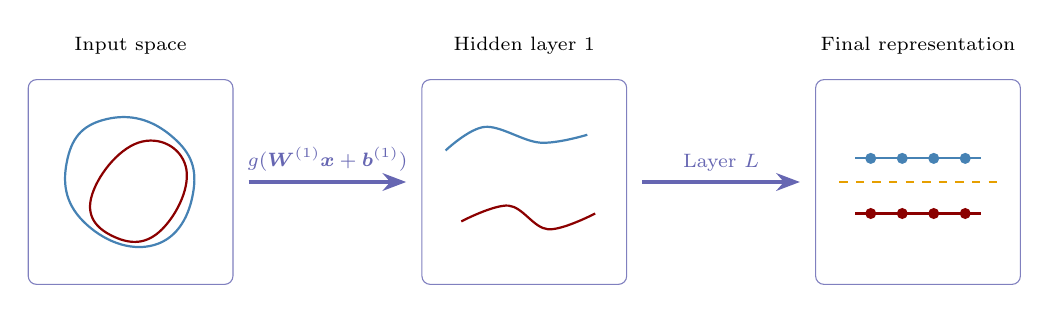
\begin{tikzpicture}[
    box/.style={rectangle, draw=uzhblue!50, rounded corners=3pt,
                minimum width=2.6cm, minimum height=2.6cm, inner sep=0pt},
    arr/.style={-{Stealth[length=3mm]}, very thick, uzhblue!60}
]
    % Panel 1: tangled
    \node[box] (p1) at (0,0) {};
    \node[font=\scriptsize, above] at (0,1.5) {Input space};
    % Draw tangled pattern
    \draw[softblue, thick] plot[smooth cycle, tension=0.8] coordinates {
        (-0.8,0.3) (-0.3,0.8) (0.5,0.6) (0.8,-0.1) (0.3,-0.8) (-0.6,-0.5)};
    \draw[darkred, thick] plot[smooth cycle, tension=0.8] coordinates {
        (-0.5,-0.2) (0.1,0.5) (0.7,0.2) (0.4,-0.6) (-0.2,-0.7)};

    % Arrow 1
    \draw[arr] (1.5,0) -- node[above, font=\scriptsize]{$g(\W^{(1)}\x+\bb^{(1)})$} (3.5,0);

    % Panel 2: partially untangled
    \node[box] (p2) at (5,0) {};
    \node[font=\scriptsize, above] at (5,1.5) {Hidden layer 1};
    \draw[softblue, thick] plot[smooth, tension=0.6] coordinates {
        (4.0,0.4) (4.5,0.7) (5.2,0.5) (5.8,0.6)};
    \draw[darkred, thick] plot[smooth, tension=0.6] coordinates {
        (4.2,-0.5) (4.8,-0.3) (5.3,-0.6) (5.9,-0.4)};

    % Arrow 2
    \draw[arr] (6.5,0) -- node[above, font=\scriptsize]{Layer $L$} (8.5,0);

    % Panel 3: linearly separable
    \node[box] (p3) at (10,0) {};
    \node[font=\scriptsize, above] at (10,1.5) {Final representation};
    % Separated
    \draw[softblue, thick] (9.2,0.3) -- (10.8,0.3);
    \fill[softblue] (9.4,0.3) circle (2pt);
    \fill[softblue] (9.8,0.3) circle (2pt);
    \fill[softblue] (10.2,0.3) circle (2pt);
    \fill[softblue] (10.6,0.3) circle (2pt);
    \draw[darkred, thick] (9.2,-0.4) -- (10.8,-0.4);
    \fill[darkred] (9.4,-0.4) circle (2pt);
    \fill[darkred] (9.8,-0.4) circle (2pt);
    \fill[darkred] (10.2,-0.4) circle (2pt);
    \fill[darkred] (10.6,-0.4) circle (2pt);
    % Separating line
    \draw[softorange, thick, dashed] (9.0,0) -- (11.0,0);
\end{tikzpicture}
\end{center}

\vspace{0.2cm}
{\small Analogy (Chollet, 2017): imagine crumpling two sheets of colored paper into a ball. A neural network learns how to smooth them out again, layer by layer, until a simple linear classifier can separate the colors.}
\end{frame}

% --- The Crumpling Analogy ---
\begin{frame}{The Paper-Crumpling Analogy (Chollet, 2017)}
\begin{columns}[c]
\column{0.55\textwidth}
\begin{center}

\includegraphics[width=\textwidth]{figures/crumple.png}
\end{center}

\column{0.42\textwidth}
Each layer of a deep network applies a simple geometric transformation:
\begin{itemize}
    \item \textbf{Affine map} $\W\x + \bb$ (rotation, scaling, translation)
    \item \textbf{Activation} $g(\cdot)$ (folding, warping)
\end{itemize}

\vspace{0.3cm}
Together, many layers ``uncrumple'' the data manifold until the classes become linearly separable.
\end{columns}
\end{frame}
\begin{frame}{}
\begin{center}
{\Huge \textcolor{uzhblue}{Part III}}\\[0.8em]
{\LARGE Training: Loss, Gradients, and Optimization}
\end{center}
\end{frame}
\begin{frame}{Gradient Descent -- The Idea}
\begin{columns}[T]
\column{0.48\textwidth}
\textbf{Goal:} find weights that minimize the loss:
\[
    \bm{\theta}^{*} = \argmin_{\bm{\theta}}\; J(\bm{\theta})
\]

\textbf{Strategy:} start from a random point, repeatedly step in the direction of steepest descent:
\[
    \bm{\theta} \;\leftarrow\; \bm{\theta} - \eta\,\nabla_{\!\bm{\theta}} J(\bm{\theta})
\]

where $\eta > 0$ is the \textbf{learning rate}.

\column{0.48\textwidth}
\begin{center}
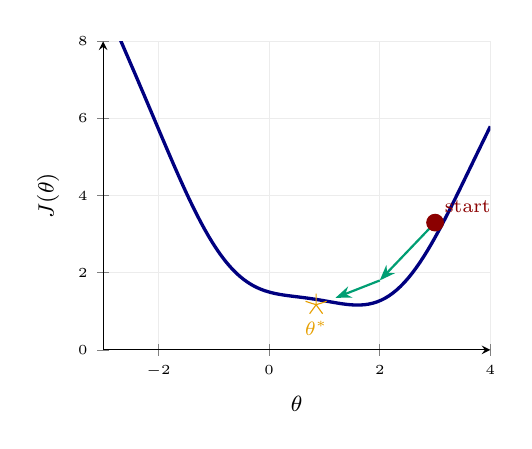
\begin{tikzpicture}
\begin{axis}[
    width=6.5cm, height=5.5cm,
    xlabel={$\theta$}, ylabel={$J(\theta)$},
    xlabel style={font=\footnotesize},
    ylabel style={font=\footnotesize},
    tick label style={font=\tiny},
    xmin=-3, xmax=4, ymin=0, ymax=8,
    grid=major, grid style={gray!15},
    axis lines=left,
    ytick={0,2,4,6,8},
]
    % Loss curve
    \addplot[very thick, uzhblue, domain=-3:4, samples=100]{0.5*(x-1)^2 + 0.3*sin(deg(x*2)) + 1};
    % Starting point
    \addplot[only marks, mark=*, mark size=3pt, darkred] coordinates {(3, 3.3)};
    \node[font=\scriptsize, darkred, above right] at (axis cs:3,3.3) {start};
    % Arrow showing descent
    \draw[-{Stealth[length=2mm]}, thick, softgreen] (axis cs:3,3.3) -- (axis cs:2,1.8);
    \draw[-{Stealth[length=2mm]}, thick, softgreen] (axis cs:2,1.8) -- (axis cs:1.2,1.35);
    % Minimum
    \addplot[only marks, mark=star, mark size=4pt, softorange] coordinates {(0.85, 1.17)};
    \node[font=\scriptsize, softorange, below] at (axis cs:0.85,1.0) {$\theta^*$};
\end{axis}
\end{tikzpicture}
\end{center}
\end{columns}
\end{frame}

% --- Slide 30: GD Algorithm ---
\begin{frame}{Gradient Descent Algorithm}
\begin{columns}[T]
\column{0.55\textwidth}
\begin{algorithm}[H]
\caption*{\textbf{Gradient Descent}}
\begin{algorithmic}[1]
\STATE Initialize $\bm{\theta} \sim \mathcal{N}(\bm{0}, \sigma^2\bm{I})$
\REPEAT
    \STATE Compute gradient: $\bm{g} \leftarrow \nabla_{\!\bm{\theta}} J(\bm{\theta})$
    \STATE Update weights: $\bm{\theta} \leftarrow \bm{\theta} - \eta\,\bm{g}$
\UNTIL{convergence}
\RETURN $\bm{\theta}$
\end{algorithmic}
\end{algorithm}

\column{0.42\textwidth}
\textbf{Key considerations:}
\begin{itemize}
    \item Computing $\nabla J$ over \emph{all} $n$ training points is $O(n)$ per step, expensive for large datasets.
    \item The learning rate $\eta$ controls step size.
    \item Convergence is to a \textbf{local} minimum (loss landscapes are non-convex for neural networks).
\end{itemize}
\end{columns}
\end{frame}

% --- Slide 31: SGD ---
\begin{frame}{Stochastic Gradient Descent (SGD)}
\textbf{Idea:} approximate the full gradient with a cheap estimate from a small subset of data.

\vspace{0.3cm}
\begin{columns}[T]
\column{0.48\textwidth}
\begin{block}{Single-sample SGD}
Pick one random example $(\x^{(i)},y^{(i)})$:
\[
    \bm{\theta} \leftarrow \bm{\theta} - \eta\,\nabla_{\!\bm{\theta}} J_i(\bm{\theta})
\]
Cheap but noisy.
\end{block}

\column{0.48\textwidth}
\begin{block}{Mini-batch SGD}
Sample a batch $\mathcal{B}$ of $B$ examples:
\[
    \bm{\theta} \leftarrow \bm{\theta} - \frac{\eta}{B}\sum_{k\in\mathcal{B}} \nabla_{\!\bm{\theta}} J_k(\bm{\theta})
\]
Reduces variance; enables GPU parallelism.
\end{block}
\end{columns}

\vspace{0.15cm}
{\small\textbf{Why does this work?} The mini-batch gradient is an \textbf{unbiased estimate} of the full gradient:}
\vspace{-0.15cm}
\[
    \E{\frac{1}{B}\sum_{k\in\mathcal{B}}\nabla J_k} = \nabla J
\]
\vspace{-0.4cm}

{\small Unbiased estimates suffice for convergence (Robbins \& Monro, 1951).}
\end{frame}

% --- Slide 32: Mini-batches and Epochs ---
\begin{frame}{Mini-Batches and Epochs}
\begin{center}
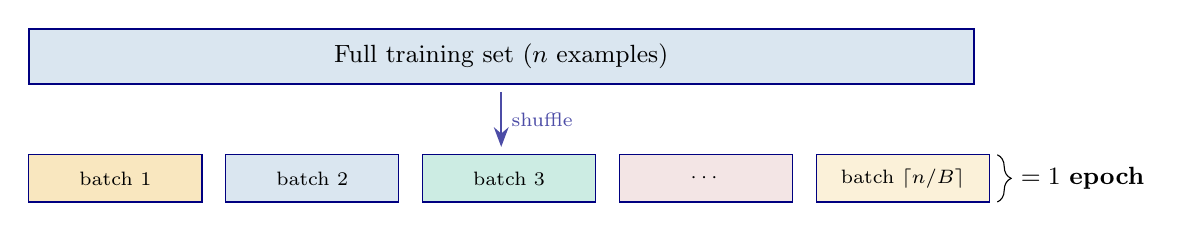
\begin{tikzpicture}[
    box/.style={rectangle, draw=uzhblue, rounded corners=3pt, minimum height=8mm, font=\small, inner sep=4pt},
    arr/.style={-{Stealth[length=2.5mm]}, thick, uzhblue!70}
]
    % Training data bar
    \fill[softblue!20] (0,0) rectangle (12,0.7);
    \draw[uzhblue, thick] (0,0) rectangle (12,0.7);
    \node[font=\small] at (6, 0.35) {Full training set ($n$ examples)};

    % Shuffle arrow
    \draw[arr] (6,-0.1) -- (6,-0.8) node[right, font=\scriptsize, pos=0.5]{shuffle};

    % Mini-batches
    \foreach \i/\c in {0/softorange!25, 2.5/softblue!20, 5/softgreen!20, 7.5/darkred!10, 10/softorange!15} {
        \fill[\c] (\i,-1.5) rectangle (\i+2.2,-0.9);
        \draw[uzhblue] (\i,-1.5) rectangle (\i+2.2,-0.9);
    }
    \node[font=\scriptsize] at (1.1,-1.2) {batch 1};
    \node[font=\scriptsize] at (3.6,-1.2) {batch 2};
    \node[font=\scriptsize] at (6.1,-1.2) {batch 3};
    \node[font=\scriptsize] at (8.6,-1.2) {$\cdots$};
    \node[font=\scriptsize] at (11.1,-1.2) {batch $\lceil n/B\rceil$};

    % Brace for epoch
    \draw[decorate, decoration={brace, amplitude=5pt}] (12.3,-0.9) -- (12.3,-1.5)
        node[midway, right=5pt, font=\small]{$= 1$ \textbf{epoch}};
\end{tikzpicture}
\end{center}

\vspace{0.5cm}
\begin{itemize}
    \item One \textbf{epoch} = one complete pass through the training set.
    \item Typical batch sizes: $B \in \{32, 64, 128, 256\}$.
    \item Benefits of mini-batches:
    \begin{itemize}
        \item[\textendash] Smoother convergence than single-sample SGD.
        \item[\textendash] Efficient use of GPU parallelism.
        \item[\textendash] Implicit regularization from gradient noise.
    \end{itemize}
\end{itemize}
\end{frame}

% --- Slide 33: Backpropagation Key Idea ---
\begin{frame}{Backpropagation -- The Key Idea}
\textbf{Problem:} how do we compute $\frac{\partial J}{\partial \W^{(\ell)}}$ for each layer $\ell$?

\vspace{0.3cm}
\textbf{Answer:} the \textbf{chain rule} of calculus, applied systematically.

\vspace{0.4cm}
\begin{center}
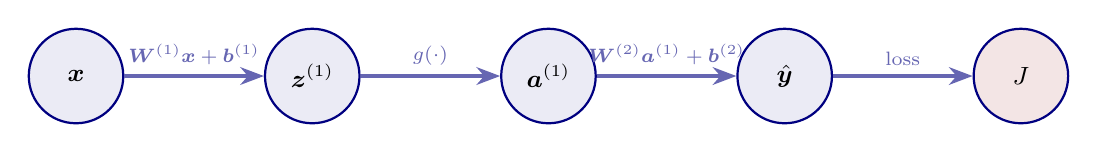
\begin{tikzpicture}[
    node/.style={circle, draw=uzhblue, thick, minimum size=12mm, fill=uzhblue!8, font=\small},
    arr/.style={-{Stealth[length=3mm]}, very thick, uzhblue!60}
]
    \node[node] (x) at (0,0) {$\x$};
    \node[node] (z1) at (3,0) {$\z^{(1)}$};
    \node[node] (a1) at (6,0) {$\a^{(1)}$};
    \node[node] (yhat) at (9,0) {$\hat{\bm{y}}$};
    \node[node, fill=darkred!10] (J) at (12,0) {$J$};

    \draw[arr] (x) -- node[above, font=\scriptsize]{$\W^{(1)}\x+\bb^{(1)}$} (z1);
    \draw[arr] (z1) -- node[above, font=\scriptsize]{$g(\cdot)$} (a1);
    \draw[arr] (a1) -- node[above, font=\scriptsize]{$\W^{(2)}\a^{(1)}+\bb^{(2)}$} (yhat);
    \draw[arr] (yhat) -- node[above, font=\scriptsize]{loss} (J);
\end{tikzpicture}
\end{center}

\vspace{0.3cm}
\[
    \frac{\partial J}{\partial \W^{(1)}} = \underbrace{\frac{\partial J}{\partial \hat{\bm{y}}}}_{\text{output error}} \cdot \underbrace{\frac{\partial \hat{\bm{y}}}{\partial \a^{(1)}}}_{\W^{(2)}} \cdot \underbrace{\frac{\partial \a^{(1)}}{\partial \z^{(1)}}}_{g'(\z^{(1)})} \cdot \underbrace{\frac{\partial \z^{(1)}}{\partial \W^{(1)}}}_{\x}
\]
\end{frame}

% --- Slide 34: Backpropagation Forward Pass ---
\begin{frame}{Backpropagation -- Forward Pass}
Given input $\x$, compute layer by layer and \textbf{store all intermediate quantities}:

\vspace{0.3cm}
\begin{center}
\renewcommand{\arraystretch}{1.4}
\begin{tabular}{rll}
\toprule
\textbf{Layer} & \textbf{Pre-activation} & \textbf{Activation} \\
\midrule
$\ell = 0$ & & $\a^{(0)} = \x$ \\
$\ell = 1$ & $\z^{(1)} = \W^{(1)}\a^{(0)} + \bb^{(1)}$ & $\a^{(1)} = g(\z^{(1)})$ \\
$\ell = 2$ & $\z^{(2)} = \W^{(2)}\a^{(1)} + \bb^{(2)}$ & $\a^{(2)} = g(\z^{(2)})$ \\
$\vdots$ & $\vdots$ & $\vdots$ \\
$\ell = L$ & $\z^{(L)} = \W^{(L)}\a^{(L-1)} + \bb^{(L)}$ & $\hat{\bm{y}} = g_{\text{out}}(\z^{(L)})$ \\
\bottomrule
\end{tabular}
\end{center}

\vspace{0.2cm}
Finally compute the loss: $J = \ell\big(\bm{y},\, \hat{\bm{y}}\big)$.
We need all the $\z^{(\ell)}$ and $\a^{(\ell)}$ values for the backward pass.
\end{frame}

% --- Slide 35: Backpropagation Backward Pass ---
\begin{frame}{Backpropagation -- Backward Pass}
Define the \textbf{error signal} at layer $\ell$:
\[
    \bm{\delta}^{(\ell)} \;\equiv\; \frac{\partial J}{\partial \z^{(\ell)}} \;\in\;\R^{n_\ell}
\]

\vspace{0.2cm}
\textbf{Output layer} ($\ell = L$):
\[
    \bm{\delta}^{(L)} = \nabla_{\!\z^{(L)}} J = \frac{\partial J}{\partial \hat{\bm{y}}}\odot g_{\text{out}}'(\z^{(L)})
\]

\textbf{Hidden layers} ($\ell = L{-}1, \dots, 1$)~~---~~propagate error \textit{backward}:
\[
    \boxed{\bm{\delta}^{(\ell)} = \big(\W^{(\ell+1)}\big)^{\!\top}\bm{\delta}^{(\ell+1)} \;\odot\; g'\!\big(\z^{(\ell)}\big)}
\]

\textbf{Parameter gradients:}
\[
    \frac{\partial J}{\partial \W^{(\ell)}} = \bm{\delta}^{(\ell)}\big(\a^{(\ell-1)}\big)^{\!\top}, \qquad
    \frac{\partial J}{\partial \bb^{(\ell)}} = \bm{\delta}^{(\ell)}
\]

{\small The symbol $\odot$ denotes the element-wise (Hadamard) product.}
\end{frame}

% --- Slide 36: Learning Rate ---
\begin{frame}{The Learning Rate}
\begin{center}
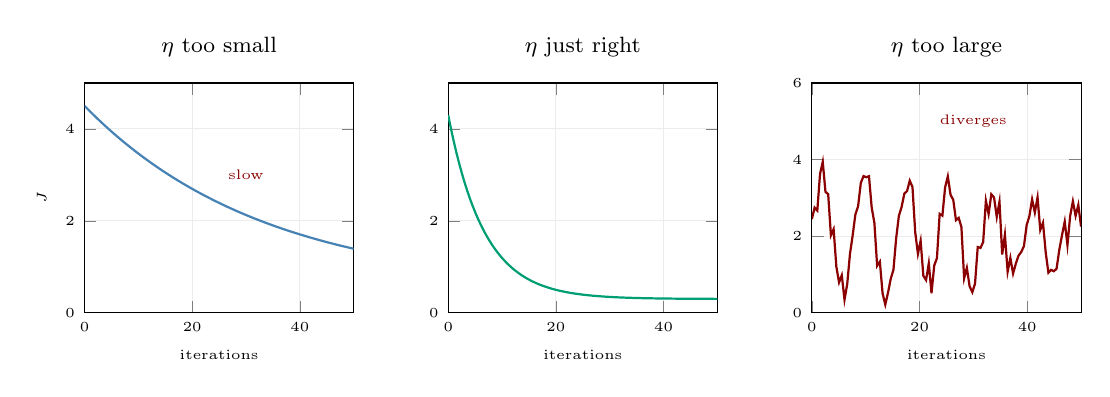
\begin{tikzpicture}
\begin{axis}[
    name=plotL,
    width=5cm, height=4.5cm,
    title={\footnotesize $\eta$ too small},
    title style={font=\footnotesize},
    xlabel={iterations}, ylabel={$J$},
    xlabel style={font=\tiny}, ylabel style={font=\tiny},
    tick label style={font=\tiny},
    xmin=0, xmax=50, ymin=0, ymax=5,
    grid=major, grid style={gray!15},
]
    \addplot[thick, softblue, domain=0:50, samples=100]{4*exp(-0.03*x)+0.5};
    \node[font=\tiny, darkred] at (axis cs:30,3) {slow};
\end{axis}

\begin{axis}[
    at={($(plotL.east)+(1.2cm,0)$)}, anchor=west,
    name=plotM,
    width=5cm, height=4.5cm,
    title={\footnotesize $\eta$ just right},
    title style={font=\footnotesize},
    xlabel={iterations},
    xlabel style={font=\tiny},
    tick label style={font=\tiny},
    xmin=0, xmax=50, ymin=0, ymax=5,
    grid=major, grid style={gray!15},
]
    \addplot[thick, softgreen, domain=0:50, samples=100]{4*exp(-0.15*x)+0.3};
\end{axis}

\begin{axis}[
    at={($(plotM.east)+(1.2cm,0)$)}, anchor=west,
    width=5cm, height=4.5cm,
    title={\footnotesize $\eta$ too large},
    title style={font=\footnotesize},
    xlabel={iterations},
    xlabel style={font=\tiny},
    tick label style={font=\tiny},
    xmin=0, xmax=50, ymin=0, ymax=6,
    grid=major, grid style={gray!15},
]
    \addplot[thick, darkred, domain=0:50, samples=100]{2+1.5*sin(deg(x*0.8))*exp(-0.01*x)+0.5*rand};
    \node[font=\tiny, darkred] at (axis cs:30,5) {diverges};
\end{axis}
\end{tikzpicture}
\end{center}

\vspace{0.3cm}
\begin{itemize}
    \item \textbf{Too small:} slow convergence, may get stuck in poor local minima.
    \item \textbf{Too large:} oscillation or divergence, overshooting the minimum.
    \item \textbf{Solution:} use \textbf{adaptive learning rates} that adjust automatically.
\end{itemize}
\end{frame}

% --- Intermezzo: Hands-on (GD / SGD / learning rate) ---
\begin{frame}{Intermezzo -- Hands-On}
\begin{block}{Gradient Descent Notebook}
Open and work through: \textbf{lecture\_03\_B02\_02\_GradientDescent\_and\_StochasticGradientDescent.ipynb}
\end{block}

\vspace{0.5cm}
\textbf{In this notebook, you will:}
\begin{enumerate}
    \item Implement gradient descent from scratch for a simple function.
    \item Compare full-batch GD with stochastic and mini-batch variants.
    \item Visualize how the learning rate affects convergence.
\end{enumerate}

\vspace{0.5cm}
\begin{center}
\textbf{Platform:}~~\url{https://nuvolos.cloud}\\[4pt]
{\small Log in and launch the ``Deep Learning for Econ'' application.}
\end{center}
\end{frame}

% --- Slide 37: Adaptive Optimizers ---
\begin{frame}{Adaptive Optimizers}
\begin{small}
\renewcommand{\arraystretch}{1.5}
\begin{tabular}{lp{9cm}}
\toprule
\textbf{Method} & \textbf{Update rule} \\
\midrule
\textbf{Momentum} & $\bm{v}_t = \mu\,\bm{v}_{t-1} + \nabla J(\bm{\theta}_t)$;~~$\bm{\theta}_{t+1} = \bm{\theta}_t - \eta\,\bm{v}_t$ \\[2pt]
\textbf{RMSProp} & $\bm{s}_t = \beta\,\bm{s}_{t-1} + (1-\beta)(\nabla J)^2$;~~$\bm{\theta}_{t+1} = \bm{\theta}_t - \frac{\eta}{\sqrt{\bm{s}_t + \varepsilon}}\odot\nabla J$ \\[2pt]
\textbf{Adam} & $\bm{m}_t = \beta_1\bm{m}_{t-1} + (1-\beta_1)\nabla J$~~~~(1st moment) \\
& $\bm{v}_t = \beta_2\bm{v}_{t-1} + (1-\beta_2)(\nabla J)^2$~~~~(2nd moment) \\
& $\hat{\bm{m}}_t = \bm{m}_t/(1-\beta_1^t)$,~~$\hat{\bm{v}}_t = \bm{v}_t/(1-\beta_2^t)$~~~~(bias correction) \\
& $\bm{\theta}_{t+1} = \bm{\theta}_t - \eta\,\hat{\bm{m}}_t \big/ (\sqrt{\hat{\bm{v}}_t} + \varepsilon)$ \\
\bottomrule
\end{tabular}
\end{small}

\vspace{0.4cm}
{\small \textbf{Adam} (Kingma \& Ba, 2015) is the most widely used default optimizer.  Typical hyperparameters: $\beta_1=0.9$, $\beta_2=0.999$, $\varepsilon=10^{-8}$.}
\end{frame}

% --- Slide 38: Weight Initialization ---
\begin{frame}{Weight Initialization}
\textbf{Why not initialize all weights to zero?}
All neurons would compute the same output $\Rightarrow$ same gradient $\Rightarrow$ symmetry is never broken.

\vspace{0.2cm}
\textbf{Random initialization:} draw weights from a distribution scaled to the layer width $n_\ell$ (the number of neurons in layer~$\ell$; $n_{\ell-1}$ is then the fan-in from the previous layer).

\vspace{0.2cm}
\begin{columns}[T]
\column{0.48\textwidth}
\begin{block}{Xavier / Glorot (2010)}
For sigmoid or tanh activations:
\[
    W_{ij}^{(\ell)} \sim \mathcal{N}\!\left(0,\; \frac{2}{n_{\ell-1} + n_{\ell}}\right)
\]
Keeps variance of activations approximately constant across layers.
\end{block}

\column{0.48\textwidth}
\begin{block}{He (2015)}
For ReLU activations:
\[
    W_{ij}^{(\ell)} \sim \mathcal{N}\!\left(0,\; \frac{2}{n_{\ell-1}}\right)
\]
Accounts for the fact that ReLU kills half the variance (negative inputs map to zero).
\end{block}
\end{columns}

\vspace{0.15cm}
{\small Biases are typically initialized to zero. Proper initialization is critical for training deep networks.}
\end{frame}

% --- Slide 39: Vanishing and Exploding Gradients ---
\begin{frame}{Vanishing and Exploding Gradients}
\begin{columns}[T]
\column{0.52\textwidth}
The backward pass multiplies through many layers:
\[
    \bm{\delta}^{(\ell)} = \big(\W^{(\ell+1)}\big)^{\!\top}\bm{\delta}^{(\ell+1)}\odot g'(\z^{(\ell)})
\]

\begin{itemize}
    \item $|g'(z)| < 1$ at every layer $\Rightarrow$ product shrinks exponentially: \textbf{vanishing gradients}
    \item $|g'(z)| > 1$ or $\|\W^{(\ell)}\|$ large $\Rightarrow$ \textbf{exploding gradients}
\end{itemize}

\vspace{0.2cm}
\textbf{Remedies:} ReLU ($g'\in\{0,1\}$), proper initialization (He/Xavier), batch normalization, gradient clipping.

\column{0.45\textwidth}
\begin{center}
{\small\textbf{Sigmoid saturation zones}}
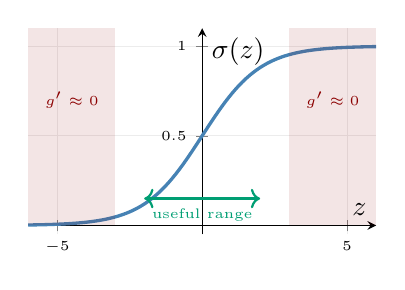
\begin{tikzpicture}
\begin{axis}[
    width=6cm, height=4.2cm,
    xlabel={$z$}, ylabel={$\sigma(z)$},
    xlabel style={font=\footnotesize},
    ylabel style={font=\footnotesize},
    tick label style={font=\tiny},
    xmin=-6, xmax=6, ymin=-0.05, ymax=1.1,
    grid=major, grid style={gray!15},
    axis lines=middle,
]
    \addplot[very thick, softblue, domain=-6:6, samples=100]{1/(1+exp(-x))};
    % Saturation zones
    \fill[darkred, opacity=0.1] (axis cs:-6,0) rectangle (axis cs:-3,1.1);
    \fill[darkred, opacity=0.1] (axis cs:3,0) rectangle (axis cs:6,1.1);
    \node[font=\tiny, darkred] at (axis cs:-4.5,0.7) {$g' \approx 0$};
    \node[font=\tiny, darkred] at (axis cs:4.5,0.7) {$g' \approx 0$};
    \draw[<->, thick, softgreen] (axis cs:-2,0.15) -- (axis cs:2,0.15)
        node[midway, below, font=\tiny]{useful range};
\end{axis}
\end{tikzpicture}
\end{center}
\end{columns}
\end{frame}

% --- Batch Normalization (a mitigation for vanishing/exploding activations) ---
\begin{frame}{Batch Normalization}
\textbf{Idea} (Ioffe \& Szegedy, 2015): normalize activations within each mini-batch to stabilize training.

\vspace{0.2cm}
For a mini-batch $\mathcal{B} = \{z_1, \dots, z_B\}$ at some layer:
\begin{align*}
    \mu_{\mathcal{B}} = \frac{1}{B}\sum_{i=1}^{B} z_i, \quad
    \sigma_{\mathcal{B}}^2 = \frac{1}{B}\sum_{i=1}^{B} (z_i - \mu_{\mathcal{B}})^2, \quad
    \hat{z}_i = \frac{z_i - \mu_{\mathcal{B}}}{\sqrt{\sigma_{\mathcal{B}}^2 + \varepsilon}}, \quad
    y_i = \gamma\, \hat{z}_i + \beta
\end{align*}

where $\gamma$ and $\beta$ are \textbf{learnable} scale and shift parameters.

\vspace{0.2cm}
\textbf{Benefits:}
\begin{itemize}
    \item Stabilizes training, allows higher learning rates.
    \item Mitigates vanishing/exploding activations across layers.
    \item Applied per-layer, typically before the activation function.
\end{itemize}

\vspace{0.1cm}
{\scriptsize \emphc{Variants beyond batch.}  LayerNorm, GroupNorm, and WeightNorm address the small-batch and recurrent settings; the script (\S\,Normalization Variants) treats them in detail.}
\end{frame}

% --- Batch Normalization: Intuition ---
\begin{frame}{Batch Normalization: Intuition}
\begin{columns}[T]
\column{0.52\textwidth}
\textbf{Why does BN help?}
\begin{itemize}\itemsep3pt
    \item[\textcolor{harvardcrimson}{$\blacktriangleright$}] {\small \emphc{The problem.} As earlier layers update, layer~$\ell$'s input distribution \emph{drifts} every step. Each layer chases a \textit{moving target} $\Rightarrow$ unstable gradients (\textit{internal covariate shift}).}
    \item[\textcolor{harvardcrimson}{$\blacktriangleright$}] {\small \emphc{The fix.} BN = standardize pre-activations every mini-batch (just like standardizing regressors). Each layer always sees inputs at $\mu{=}0,\sigma{=}1$ $\Rightarrow$ gradients flow predictably, larger learning rates become safe.}
    \item[\textcolor{harvardcrimson}{$\blacktriangleright$}] {\small \emphc{Why $\gamma,\beta$?} They are learnable: a layer that prefers non-standard inputs can shift them back. BN never reduces capacity, it just gives optimization a better starting point.}
\end{itemize}

\column{0.46\textwidth}
\begin{center}
{\small\textbf{Pre-activations $z$ at one hidden layer}}\\[0.05cm]

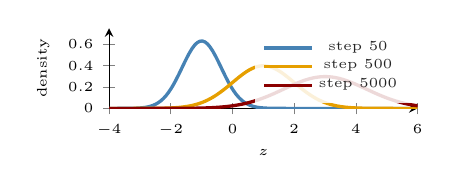
\begin{tikzpicture}
\begin{axis}[
    width=5.5cm, height=2.6cm,
    xmin=-4, xmax=6, ymin=0, ymax=0.75,
    xtick={-4,-2,0,2,4,6},
    xlabel={$z$}, xlabel style={font=\tiny, yshift=2pt},
    ylabel={density}, ylabel style={font=\tiny},
    tick label style={font=\tiny},
    axis lines=left, samples=120, no markers,
    legend style={font=\tiny, draw=none, fill=white, fill opacity=0.85,
                  at={(0.98,0.98)}, anchor=north east, row sep=-2pt}
]
    \addplot[very thick, softblue,   domain=-4:6] {1/sqrt(2*pi*0.4)*exp(-(x+1)^2/(2*0.4))};
    \addlegendentry{step 50}
    \addplot[very thick, softorange, domain=-4:6] {1/sqrt(2*pi*1.0)*exp(-(x-1)^2/(2*1.0))};
    \addlegendentry{step 500}
    \addplot[very thick, darkred,    domain=-4:6] {1/sqrt(2*pi*1.8)*exp(-(x-3)^2/(2*1.8))};
    \addlegendentry{step 5000}
\end{axis}
\end{tikzpicture}\\[-0.1cm]
{\scriptsize\itshape Without BN: distribution drifts $\to$ moving target.}

\vspace{0.2cm}
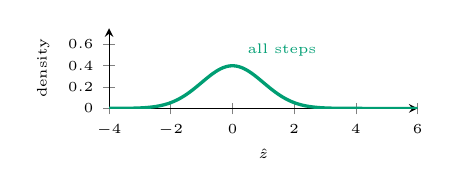
\begin{tikzpicture}
\begin{axis}[
    width=5.5cm, height=2.6cm,
    xmin=-4, xmax=6, ymin=0, ymax=0.75,
    xtick={-4,-2,0,2,4,6},
    xlabel={$\hat z$}, xlabel style={font=\tiny, yshift=2pt},
    ylabel={density}, ylabel style={font=\tiny},
    tick label style={font=\tiny},
    axis lines=left, samples=120, no markers,
]
    \addplot[very thick, softgreen, domain=-4:6] {1/sqrt(2*pi)*exp(-x^2/2)};
    \node[font=\tiny, softgreen] at (axis cs:1.6,0.55) {all steps};
\end{axis}
\end{tikzpicture}\\[-0.1cm]
{\scriptsize\itshape With BN: pinned to $\mathcal{N}(0,1)$ at every step.}
\end{center}
\end{columns}
\end{frame}
\begin{frame}{Modern Activation Functions: When to Use What}
{\footnotesize The common thread is \emphc{smoothness}. ReLU's kink at $z{=}0$ causes \textit{dead neurons} and an \textit{undefined second derivative}. Two families fix this; they differ only in whether they keep ReLU's asymptotic shape.}

\begin{columns}[T]
\column{0.55\textwidth}
\textbf{\textcolor{softblue}{Smooth \& ReLU-shaped}} {\footnotesize --- default for feedforward / CNN / attention:}
\begin{itemize}\itemsep0pt
    \item[\textcolor{softblue}{$\blacktriangleright$}] {\footnotesize \textbf{Swish/SiLU} $z\,\sigma(z)$: drop-in ReLU replacement (Ramachandran et al., 2017).}
    \item[\textcolor{harvardcrimson}{$\blacktriangleright$}] {\footnotesize \textbf{GELU} $z\,\Phi(z)$: transformer default (BERT, GPT, ViT).}
    \item[\textcolor{softgreen}{$\blacktriangleright$}] {\footnotesize \textbf{Mish} $z\tanh(\ln(1{+}e^z))$: modern vision (YOLOv4).}
\end{itemize}

\vspace{0.1cm}
\textbf{\textcolor{softorange}{Smooth, different shape}} {\footnotesize --- specialized outputs or differentiable losses:}
\begin{itemize}\itemsep0pt
    \item[\textcolor{softorange}{$\blacktriangleright$}] {\footnotesize \textbf{Softplus} $\ln(1{+}e^z)$: strictly positive $\Rightarrow$ variance heads ($\sigma^2$), Poisson rates.}
    \item[\textcolor{uzhblue}{$\blacktriangleright$}] {\footnotesize \textbf{tanh}: bounded $C^\infty$ $\Rightarrow$ PINNs (Lecture 18) where 2nd derivatives of the network enter the loss.}
\end{itemize}

\column{0.43\textwidth}
\begin{center}
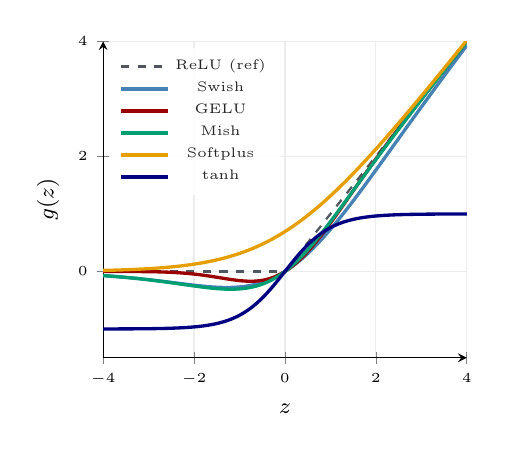
\begin{tikzpicture}
\begin{axis}[
    width=6.2cm, height=5.6cm,
    xlabel={$z$}, ylabel={$g(z)$},
    xlabel style={font=\footnotesize},
    ylabel style={font=\footnotesize},
    tick label style={font=\tiny},
    xmin=-4, xmax=4, ymin=-1.5, ymax=4,
    grid=major, grid style={gray!15},
    axis lines=left, samples=150, no markers,
    legend style={font=\tiny, draw=none, fill=white, fill opacity=0.85,
                  at={(0.02,0.98)}, anchor=north west, row sep=-1pt},
]
    % ReLU (baseline, gray dashed)
    \addplot[thick, uzhgreydark, dashed, domain=-4:0, samples=2]{0};
    \addlegendentry{ReLU (ref)}
    \addplot[thick, uzhgreydark, dashed, forget plot, domain=0:4, samples=2]{x};
    % Swish
    \addplot[very thick, softblue, domain=-4:4]{x/(1+exp(-x))};
    \addlegendentry{Swish}
    % GELU (tanh approximation)
    \addplot[very thick, harvardcrimson, domain=-4:4]
        {0.5*x*(1+tanh(0.7978845608*(x+0.044715*x*x*x)))};
    \addlegendentry{GELU}
    % Mish
    \addplot[very thick, softgreen, domain=-4:4]{x*tanh(ln(1+exp(x)))};
    \addlegendentry{Mish}
    % Softplus
    \addplot[very thick, softorange, domain=-4:4]{ln(1+exp(x))};
    \addlegendentry{Softplus}
    % tanh
    \addplot[very thick, uzhblue, domain=-4:4]{tanh(x)};
    \addlegendentry{tanh}
\end{axis}
\end{tikzpicture}
\end{center}
\end{columns}
\end{frame}
\begin{frame}{Software Ecosystem}
\begin{center}

\begin{tikzpicture}[
    fw/.style={rectangle, draw=uzhblue, fill=uzhblue!8, rounded corners=5pt,
               minimum width=3.2cm, minimum height=1.8cm, align=center, font=\small}
]
    \node[fw, fill=softorange!15] (tf) at (0,0) {\textbf{\large TensorFlow}\\+ Keras\\{\scriptsize Google, 2015}};
    \node[fw, fill=darkred!8] (pt) at (5.5,0) {\textbf{\large PyTorch}\\{\scriptsize Meta AI, 2017}};
    \node[fw, fill=softgreen!10] (jax) at (11,0) {\textbf{\large JAX}\\{\scriptsize Google, 2018}};
\end{tikzpicture}
\end{center}

\vspace{0.5cm}
\begin{itemize}
    \item \textbf{Keras} (\url{https://keras.io}) provides a high-level API that runs on top of TensorFlow, PyTorch, or JAX---write once, run anywhere.
    \item \textbf{Key resources:}
    \begin{itemize}
        \item Keras sequential model: \url{https://www.tensorflow.org/guide/keras/sequential_model}
        \item TensorBoard: \url{https://www.tensorflow.org/tensorboard}
        \item PyTorch tutorials: \url{https://pytorch.org/tutorials}
    \end{itemize}
\end{itemize}
\end{frame}
\begin{frame}{Hands-On Notebooks}
The following Jupyter notebooks are available on Nuvolos:

\vspace{0.3cm}
\begin{center}
{\scriptsize
\renewcommand{\arraystretch}{1.15}
\begin{tabular}{clp{5.2cm}}
\toprule
\textbf{\#} & \textbf{Notebook} & \textbf{Content} \\
\midrule
1 & \texttt{01\_BasicML\_intro} & Linear regression, classification, clustering, loss functions \\
2 & \texttt{02\_GradientDescent\_and\_SGD} & Gradient descent, line search, SGD, mini-batch \\
3 & \texttt{03\_Double\_Descent} & Double-descent with random Fourier features \\
4 & \texttt{04\_Gentle\_DNN} & First neural network with Keras \\
5 & \texttt{05\_Tensorboard} & Visualizing training with TensorBoard \\
6 & \texttt{06\_PyTorch\_intro} & Introduction to PyTorch \\
7 & \texttt{07\_Genz\_Approximation\_and\_Loss} & Genz functions, NN approximation, robust losses \\
8 & \texttt{08\_MLP\_LSTM\_Transformer\_Edgeworth\_Cycles} & MLP vs LSTM vs tiny Transformer on Edgeworth cycles \\
9 & \texttt{09\_Transformer\_InContext\_AR1} & Tiny transformer, in-context learning of AR(1) \\
\bottomrule
\end{tabular}
\vspace{0.2cm}\\
{\tiny File \#2: \texttt{02\_GradientDescent\_and\_StochasticGradientDescent.ipynb};\ \#7: \texttt{07\_Genz\_Approximation\_and\_Loss\_Functions.ipynb}.}
}%
\end{center}
\end{frame}
\begin{frame}{Exercise: Architecture Exploration}
\textbf{Using the Genz functions from the previous exercise:}

\vspace{0.4cm}
\begin{enumerate}
    \item \textbf{Vary the depth:} try 1, 2, 3, and 5 hidden layers.  How does depth affect approximation quality?

    \vspace{0.3cm}
    \item \textbf{Vary the activation:} compare sigmoid, tanh, ReLU, and Swish.  Which works best for smooth vs.\ discontinuous functions?

    \vspace{0.3cm}
    \item \textbf{Vary the optimizer:} compare plain SGD, SGD with momentum, and Adam.  Monitor convergence speed and final accuracy.

    \vspace{0.3cm}
    \item \textbf{Plot} the maximum and average approximation error as a function of the number of training points.  What happens as $d$ grows?
\end{enumerate}

\vspace{0.3cm}
{\small \textbf{Hint:} you should observe the ``curse of dimensionality'', the error grows significantly with $d$ for a fixed number of training points.}
\end{frame}

% --- Slide 53: Questions ---
\begin{frame}{}
\begin{columns}[c]
\column{0.45\textwidth}
\begin{center}

\includegraphics[width=0.85\textwidth]{figures/quest.png}
\end{center}

\column{0.50\textwidth}
\begin{center}
{\Huge \textcolor{uzhblue}{\textbf{Questions?}}}

\vspace{0.8cm}
{\large Simon Scheidegger}\\[4pt]
{\small HEC, University of Lausanne}\\[4pt]
\url{https://sischei.github.io}

\vspace{0.6cm}
{\small Materials:~~\url{https://github.com/sischei/Deep_Learning_for_Solving_And_Estimating_Dynamic_Economic_Models}}
\end{center}
\end{columns}
\end{frame}

\end{document}
